% !TEX TS-program = pdflatexmk
\documentclass[12pt]{article}

% Layout.
\usepackage[top=1in, bottom=0.75in, left=1in, right=1in, headheight=1in, headsep=6pt]{geometry}

% Fonts.
\usepackage{mathptmx}
\usepackage[scaled=0.86]{helvet}
\renewcommand{\emph}[1]{\textsf{\textbf{#1}}}

% TiKZ.
\usepackage{tikz, pgfplots}
\usetikzlibrary{calc}
\pgfplotsset{my style/.append style={axis x line=middle, axis y line=
middle, xlabel={$x$}, ylabel={$y$}, axis equal }}

% Misc packages.
\usepackage{amsmath,amssymb,latexsym}
\usepackage{graphicx}
\usepackage{array}
\usepackage{xcolor}
\usepackage{multicol}

% Commands to set various header/footer components.
\makeatletter
\def\doctitle#1{\gdef\@doctitle{#1}}
\doctitle{Use {\tt\textbackslash doctitle\{MY LABEL\}}.}
\def\docdate#1{\gdef\@docdate{#1}}
\docdate{Use {\tt\textbackslash docdate\{MY DATE\}}.}
\def\doccourse#1{\gdef\@doccourse{#1}}
\let\@doccourse\@empty
\def\docscoring#1{\gdef\@docscoring{#1}}
\let\@docscoring\@empty
\def\docversion#1{\gdef\@docversion{#1}}
\let\@docversion\@empty
\makeatother

% Headers and footers layout.
\makeatletter
\usepackage{fancyhdr}
\pagestyle{fancy}
\fancyhf{} % Clears all headers/footers.
\lhead{\baselineskip 30pt
\emph{\@doctitle\hfill\@docdate}
\ifnum \value{page} > 1\relax\else\\
\emph{Name: \rule{3.5in}{1pt}\hfill \@docscoring}\fi}
\rfoot{\emph{\@docversion}}
\lfoot{\emph{\@doccourse}}
\cfoot{\emph{\thepage}}
\renewcommand{\headrulewidth}{0pt}%
\makeatother

% Paragraph spacing
\parindent 0pt
\parskip 6pt plus 1pt

% A problem is a section-like command. Use \problem{5} to
% start a problem worth 5 points.
\newcounter{probcount}
\newcounter{subprobcount}
\setcounter{probcount}{0}
\newcommand{\problem}[1]{%
\par
\addvspace{4pt}%
\setcounter{subprobcount}{0}%
\stepcounter{probcount}%
\makebox[0pt][r]{\emph{\arabic{probcount}.}\hskip1ex}\emph{[#1 points]}\hskip1ex}
\newcommand{\thesubproblem}{\emph{\alph{subprobcount}.}}

% Subproblems are an enumerate-like environment with a consistent
% numbering scheme. 
% Use \begin{subproblems}\item...\item...\end{subproblems}
\newenvironment{subproblems}{%
\begin{enumerate}%
\setcounter{enumi}{\value{subprobcount}}%
\renewcommand{\theenumi}{\emph{\alph{enumi}}}}%
{\setcounter{subprobcount}{\value{enumi}}\end{enumerate}}

% Blanks for answers in normal and math mode.
\newcommand{\blank}[1]{\rule{#1}{0.75pt}}
\newcommand{\mblank}[1]{\underline{\hspace{#1}}}
\def\emptybox(#1,#2){\framebox{\parbox[c][#2]{#1}{\rule{0pt}{0pt}}}}

% Misc.
\renewcommand{\d}{\displaystyle}
\newcommand{\ds}{\displaystyle}
\def\bc{\begin{center}}
\def\ec{\end{center}}


\doctitle{Math 251: Quiz \#0 (Getting Started Quiz)}
\docdate{August 24, 2020}
\doccourse{UAF Calculus I}
\docversion{v-1}
\docscoring{\blank{0.8in} / 5}
\begin{document}
This quiz is designed to help make sure you are familiar with some important details about your Calculus I course this semester, and to help you practice some of the technology. There are also some questions to help your instructor get to know you.

You can find answers to many of these questions in the Syllabus, on the Calculus I website, and in our course Blackboard site.

\textbf{To receive full credit\footnote{Quiz 0 counts in the ``Notes/Worksheets'' category in the syllabus, but it's \emph{called} Quiz 0 because it's practice for the other quizzes you will be taking.}, you must upload your completed Quiz 0 into Gradescope by Friday August 28 by 4pm.} You probably want to try to upload it much sooner than that so you can sort out any technology issues.

\begin{enumerate} 
\item What day is your first WebAssign homework due?
\vfill
\item (Synchronous class) What day is DH4 due? (Asynchronous class) What day is your first Written Homework due?
\vfill
\item What day is the Prerequisite Quiz (Quiz 1)? Where can you find sample quizzes?
\vfill 
\item What day is Midterm 1? 
\vfill 
\item True or False? You can complete your WebAssign assignments after the due date. (Circle the correct answer.)
\vfill
\item  True or False? You can turn in your homework late. (Circle the correct answer.)
\vfill
\item  True or False? You can be withdrawn from the course for missing class and not doing your homework. (Circle the correct answer.)
\vfill
\item  True or False? You can access WebAssign and an electronic copy of the textbook for two weeks without paying. (Circle the correct answer.)
\vfill
\item Write your instructor's name: 
\vfill
\item Write your recitation leader's name: 
\vfill

\newpage

\item How much time per week should you plan to spend studying for this class outside lecture and recitation?
\vfill

%\item Go to the Math \& Stat Tutoring Lab in Chapman Hall Room Room 305 and get a tutor to print and sign his/her name below.
%\vfill
\item What are some ways you can access tutoring?
\vfill
\item What is your major? Write down a best guess even if you are not sure!
\vfill
\item How certain are you of your answer to the question 13 above? 
\vfill

\item Have you taken a calculus class before? If so, where and when? (e.g., did you take Calculus in high school?)
\vfill
\item Tell your instructor one interesting, funny, unexpected or kooky thing about yourself.
\vfill
\item (optional) Do you have anything you want to tell us (concerns, things you're excited about) for this semester? 
\vspace{2in}
\end{enumerate}

\end{document}
A population of voles is taking over a garden. The table
below indicates the size of the population measured at the middle of each week during a summer.
\begin{center}
\begin{tabular}{|c|c|c|c|c|c|c|}
\hline
$t$ (weeks) &1&2&3&4&5&6 \\
\hline
$n$ (voles) & 7& 15& 31& 63&73&82 \\
\hline
\end{tabular}
\end{center}

\begin{subproblems}
\item Find the average rate of change of the population over 
the entire measurement period.
\vskip 2cm

\item Find the average rate of change of the population
from week 3 to week 5.
\end{subproblems}
\vskip 2cm


\problem{9}
Use the graph of the function of $f(x)$ to answer the following questions.\\
\begin{center}
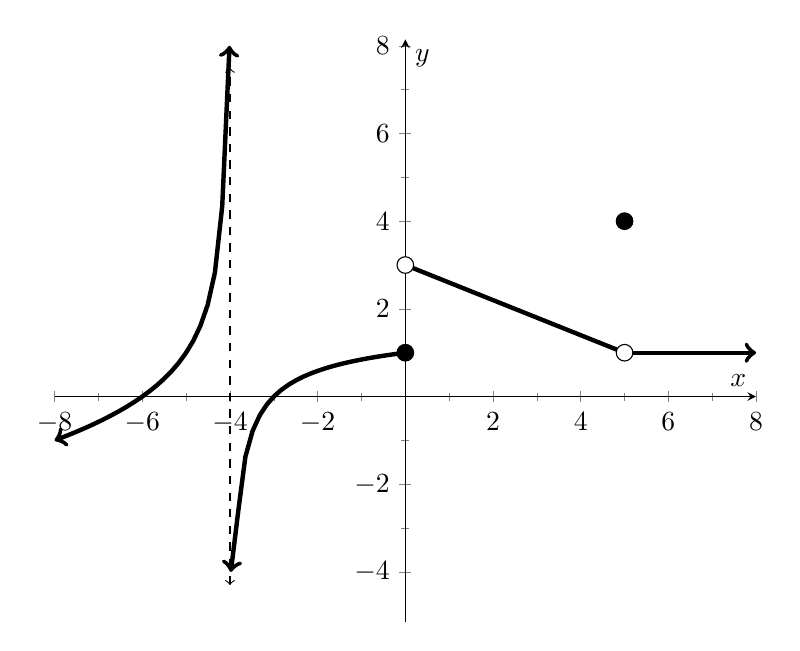
\begin{tikzpicture}
\begin{axis}[scale=1.3, my style, xtick={-8,-6,...,8}, ytick={-4,-2,...,8},
xmin=-8, xmax=8, ymin=-5, ymax=8, minor y tick num=1,
        minor x tick num=1, mark size=3.0pt]
\addplot[domain=5:8,->,ultra thick] {1};
\addplot[domain=0:5, -, ultra thick] {3 - 2*x/5 };
\addplot[domain=-3.98:0,<-, ultra thick] {max(2-2/sqrt(((4+x))),-4)};
% \addplot[domain=3:4.87,->, ultra thick]{3.5+(x-5)^(-1)};
\addplot[domain=-8:-4.01,<->, ultra thick]{min((6+x)/sqrt(-x-4),8)};
% \addplot[dotted] coordinates {(-5,3) (-5,-4)};
\addplot[dashed,<->] coordinates {(-4,-4.3) (-4,7.5)};
\addplot[mark=*,only marks] coordinates {(5,4)(0,1)};
\addplot[mark=*,fill=white,only marks] coordinates {(5,1)
(0,3)};
\end{axis}
\end{tikzpicture}
\end{center}

\begin{subproblems}
\begin{multicols}{3}
\item $\d{\lim_{x \to 0^+} f(x)=\mblank{.5in}}$
\item $\d{\lim_{x \to 0^-} f(x)=\mblank{.5in}}$
\item $\d{\lim_{x \to 0} f(x)=\mblank{.5in}}$
\end{multicols}
\begin{multicols}{3}
\item $f(0)=\mblank{.5in}$
\item $f(5)=\mblank{.5in}$
\item $f(-6)=\mblank{.5in}$
\end{multicols}
\begin{multicols}{3}
\item $\d{\lim_{x \to -4^+} f(x)=\mblank{.5in}}$
\item $\d \lim_{x\to 5}f(x)=\mblank{.5in}$
\item $\d{\lim_{x \to -6} f(x)=\mblank{.5in}}$
\end{multicols}
\end{subproblems}

\newpage
\problem{6} Compute the following limits. For each limit, justify your answer 
with a sentence or two.
\begin{subproblems}
\item$\d \lim_{x\rightarrow 8^+} \frac{2+x}{(x-8)^2}=\emptybox(40pt,30pt)$
\vskip 3cm

\item$\d \lim_{x\rightarrow \pi^+} \frac{\sqrt{2}}{\sin(x)}=\emptybox(40pt,30pt)$
\vskip 3cm
\end{subproblems}


\problem{6} On the axes below, sketch the graph of the function 
\[
f(x)=\begin{cases} 
2-x & x < 1\\
3 & x = 1\\
\frac{1}{1-x} & x>1.
\end{cases}
\]

Then compute, with brief justification, the requested values in the table.

\begin{multicols}{2}

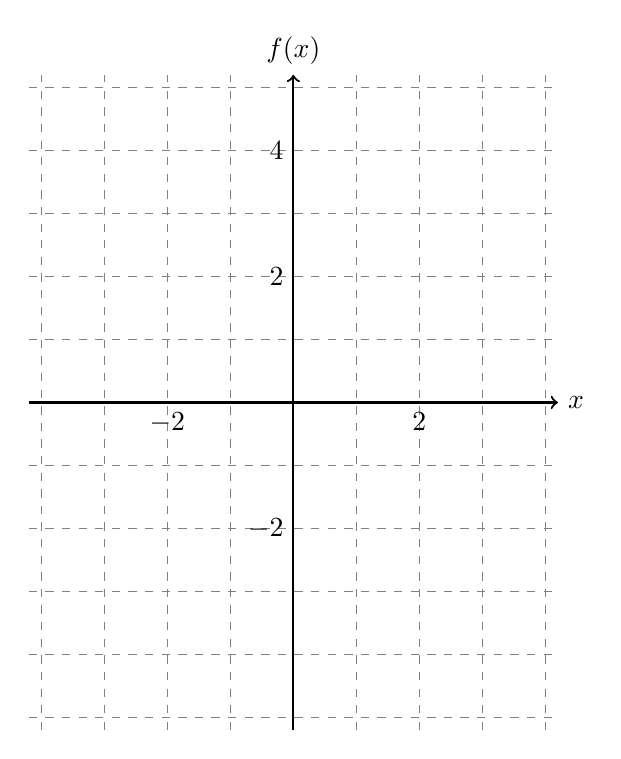
\begin{tikzpicture}[scale=0.8]
\draw [help lines,dashed] (-4.2,-5.2) grid (4.2,5.2);
\draw [thick, ->] (-4.2,0)--(4.2,0) node[right] {$x$};
\draw [thick, ->] (0,-5.2)--(0,5.2) node[above]{$f(x)$};
\foreach \i in {-2,2}
{	\node[below] at (\i,0) {$\i$};
}
\foreach \i in {-2,2,4}
{	\node[left] at (0,\i) {$\i$};
}
\end{tikzpicture}

\columnbreak

\begin{tabular}{|c|c|}\hline
Value & Justification \\ \hline
$f(1)=$ &\raisebox{10pt}{\parbox[t][0.8in]{2.5in}{\strut}}\\ \hline
$\d \lim_{x\rightarrow 1^-} f(x)=$  &\raisebox{20pt}{\parbox[t][1.2in]{2.5in}{}}\\\hline
$\d \lim_{x\rightarrow 1} f(x)=$    &\raisebox{20pt}{\parbox[t][1.2in]{2.5in}{}} \\ \hline
\end{tabular}
\end{multicols}

\end{document}
